\documentclass[tikz]{standalone}

\usepackage{xcolor}

\usetikzlibrary{positioning}

\definecolor{stgoblue}{RGB}{74,144,226}
\definecolor{stgogreen}{RGB}{80,227,194}
\definecolor{stgored}{RGB}{255,69,0}
\definecolor{stgoorange}{RGB}{255,165,0}

\begin{document}

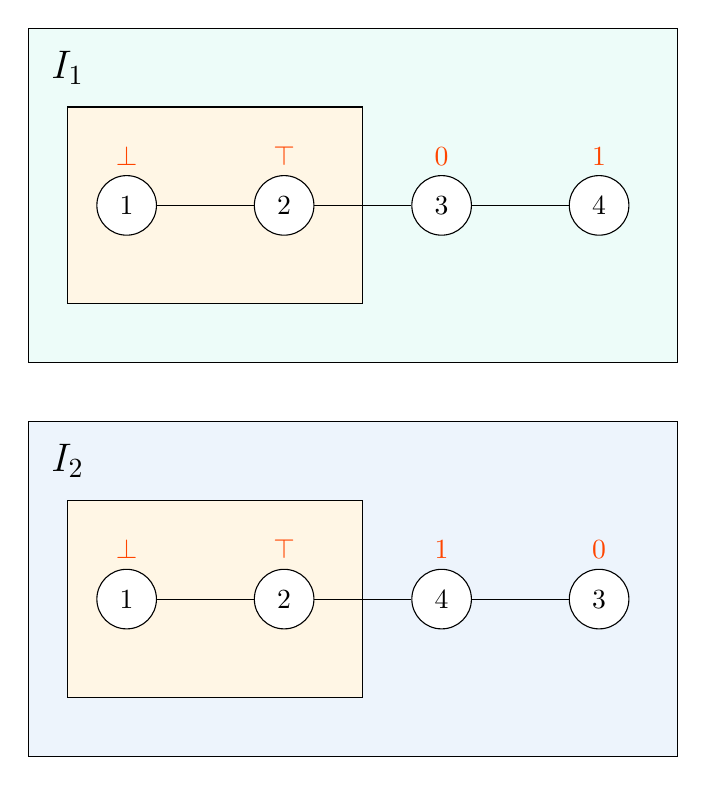
\begin{tikzpicture}
    \colorlet{colorLabel}{stgored}
    \tikzstyle{nodeStyle}=[circle, draw, fill=white, inner sep=2pt,
      minimum size=5ex]
    \tikzstyle{labelStyle}=[draw=none, minimum size=0ex, color=colorLabel]

    \draw[fill=stgogreen!10] (-1.25,2.25) rectangle (7,-2);
    \node at (-0.75,1.75) {\Large $I_1$};

    \draw[fill=stgoorange!10] (-0.75,-1.25) rectangle (3,1.25);
    
    \node[nodeStyle,label={[labelStyle]90:$\bot$}] (1) at (0,0) {$1$};
    \node[nodeStyle,label={[labelStyle]90:$\top$}] (2) at (2,0) {$2$};
    \node[nodeStyle,label={[labelStyle]90:$0$}] (3) at (4,0) {$3$};
    \node[nodeStyle,label={[labelStyle]90:$1$}] (4) at (6,0) {$4$};

    \draw (1) -- (2);
    \draw (2) -- (3);
    \draw (3) -- (4);

    \begin{scope}[shift={(0,-5)}]
      \draw[fill=stgoblue!10] (-1.25,2.25) rectangle (7,-2);
      \node at (-0.75,1.75) {\Large $I_2$};

      \draw[fill=stgoorange!10] (-0.75,-1.25) rectangle (3,1.25);
      
      \node[nodeStyle,label={[labelStyle]90:$\bot$}] (1) at (0,0) {$1$};
      \node[nodeStyle,label={[labelStyle]90:$\top$}] (2) at (2,0) {$2$};
      \node[nodeStyle,label={[labelStyle]90:$1$}] (4) at (4,0) {$4$};
      \node[nodeStyle,label={[labelStyle]90:$0$}] (3) at (6,0) {$3$};

      \draw (1) -- (2);
      \draw (2) -- (4);
      \draw (4) -- (3);
    \end{scope}
\end{tikzpicture}

\end{document}
